\chapter{Beschreibung aus Anwendersicht} \label{anwendersicht}
Dieses Projekt ist für den Kunden entwickelt worden, daher wird hier die Anwendersicht beschrieben.
\section{Länderwahl}
\begin{figure}[h]
	\centerline{
		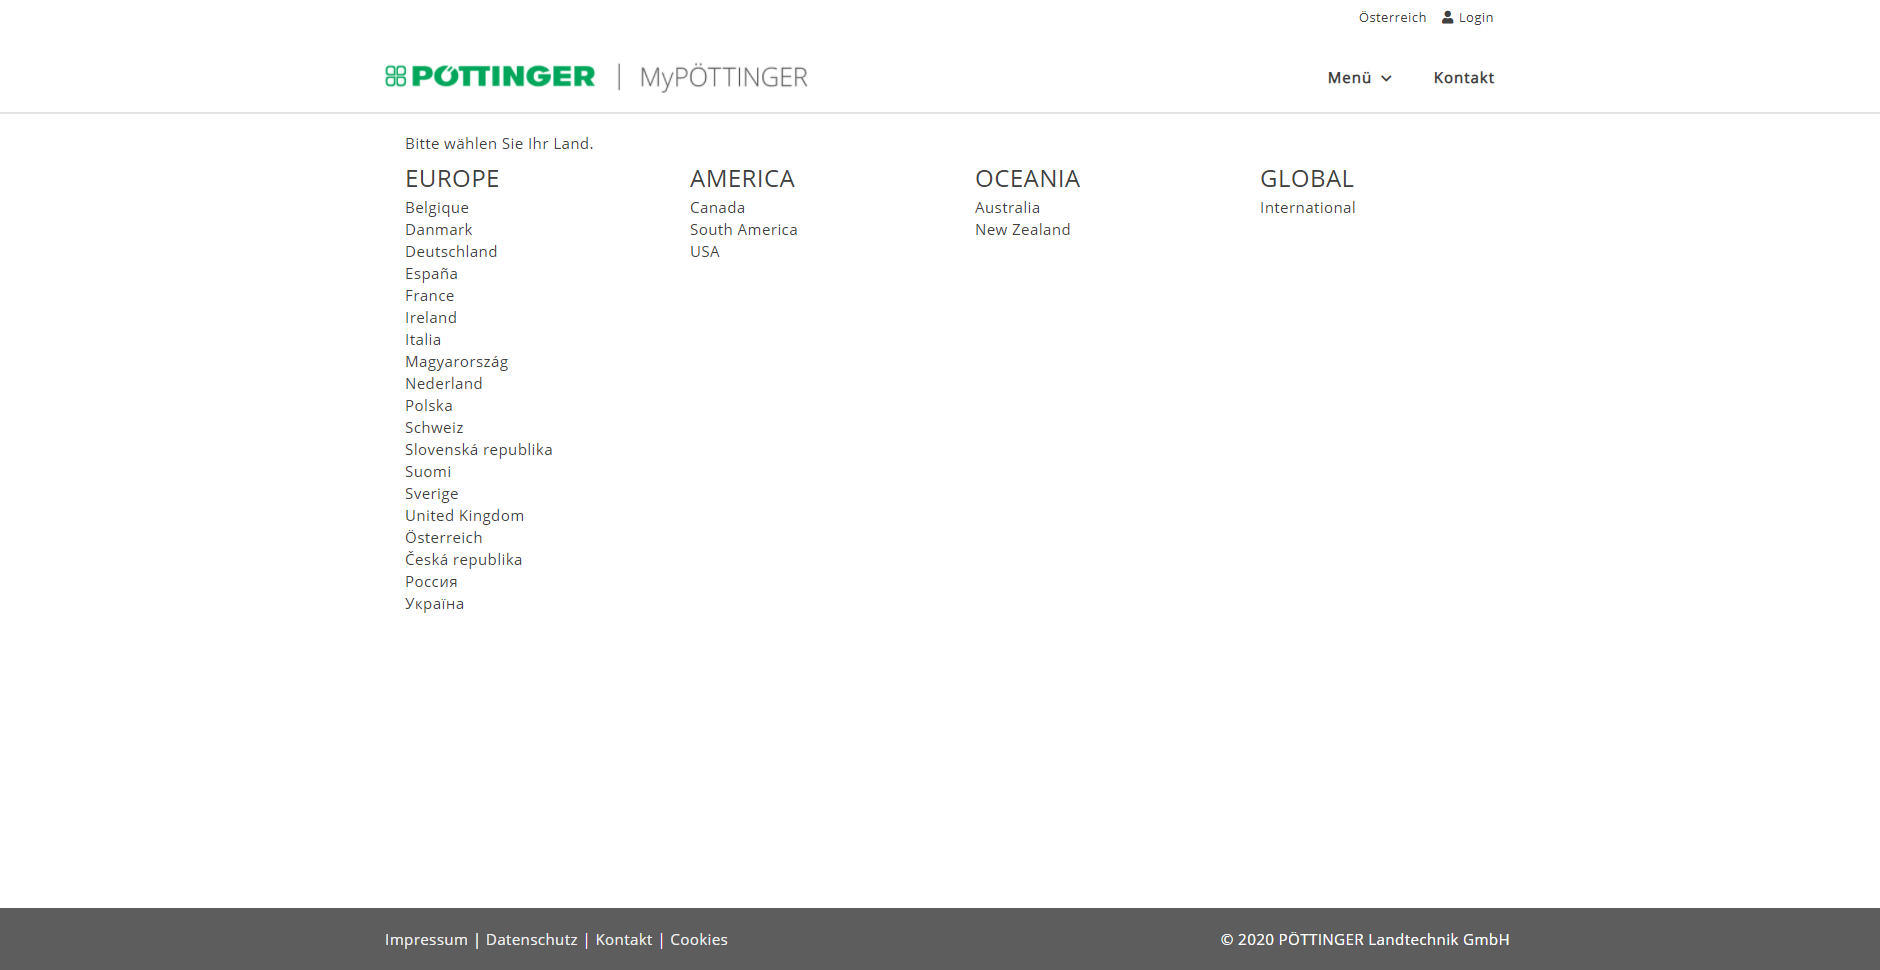
\includegraphics[width=0.8\textwidth]{./grafiken/erm_country_selection.png}
	}
	\vskip0pt
	\caption{Screenshot von Länderwahl} \label{fig:countrySelection}
\end{figure}
Um auf die Webseite zu gelangen, muss man davor in der Länderwahl sein Land und bei den Ländern, wo es mehrere Landssprachen gibt, auch die Sprache wählen. Aus dem Länder- und Sprachenkürzel setzt sich die Locale zusammen. Für Österreich wäre die Locale daher "de\_AT" und für Deutschland "de\_DE". Diese Locale wird in den Cookies gespeichert und die Webseite richtet sich nach dieser Locale in den Cookies. Es ist auch möglich, im Nachhinein das Land und die Sprache zu ändern, indem man im Header der Webseite auf das Land klickt. Durch diesen Klick gelangt man von überall auf die Länderwahl.

\section{Startseite}
\begin{figure}[H]
	\centerline{
		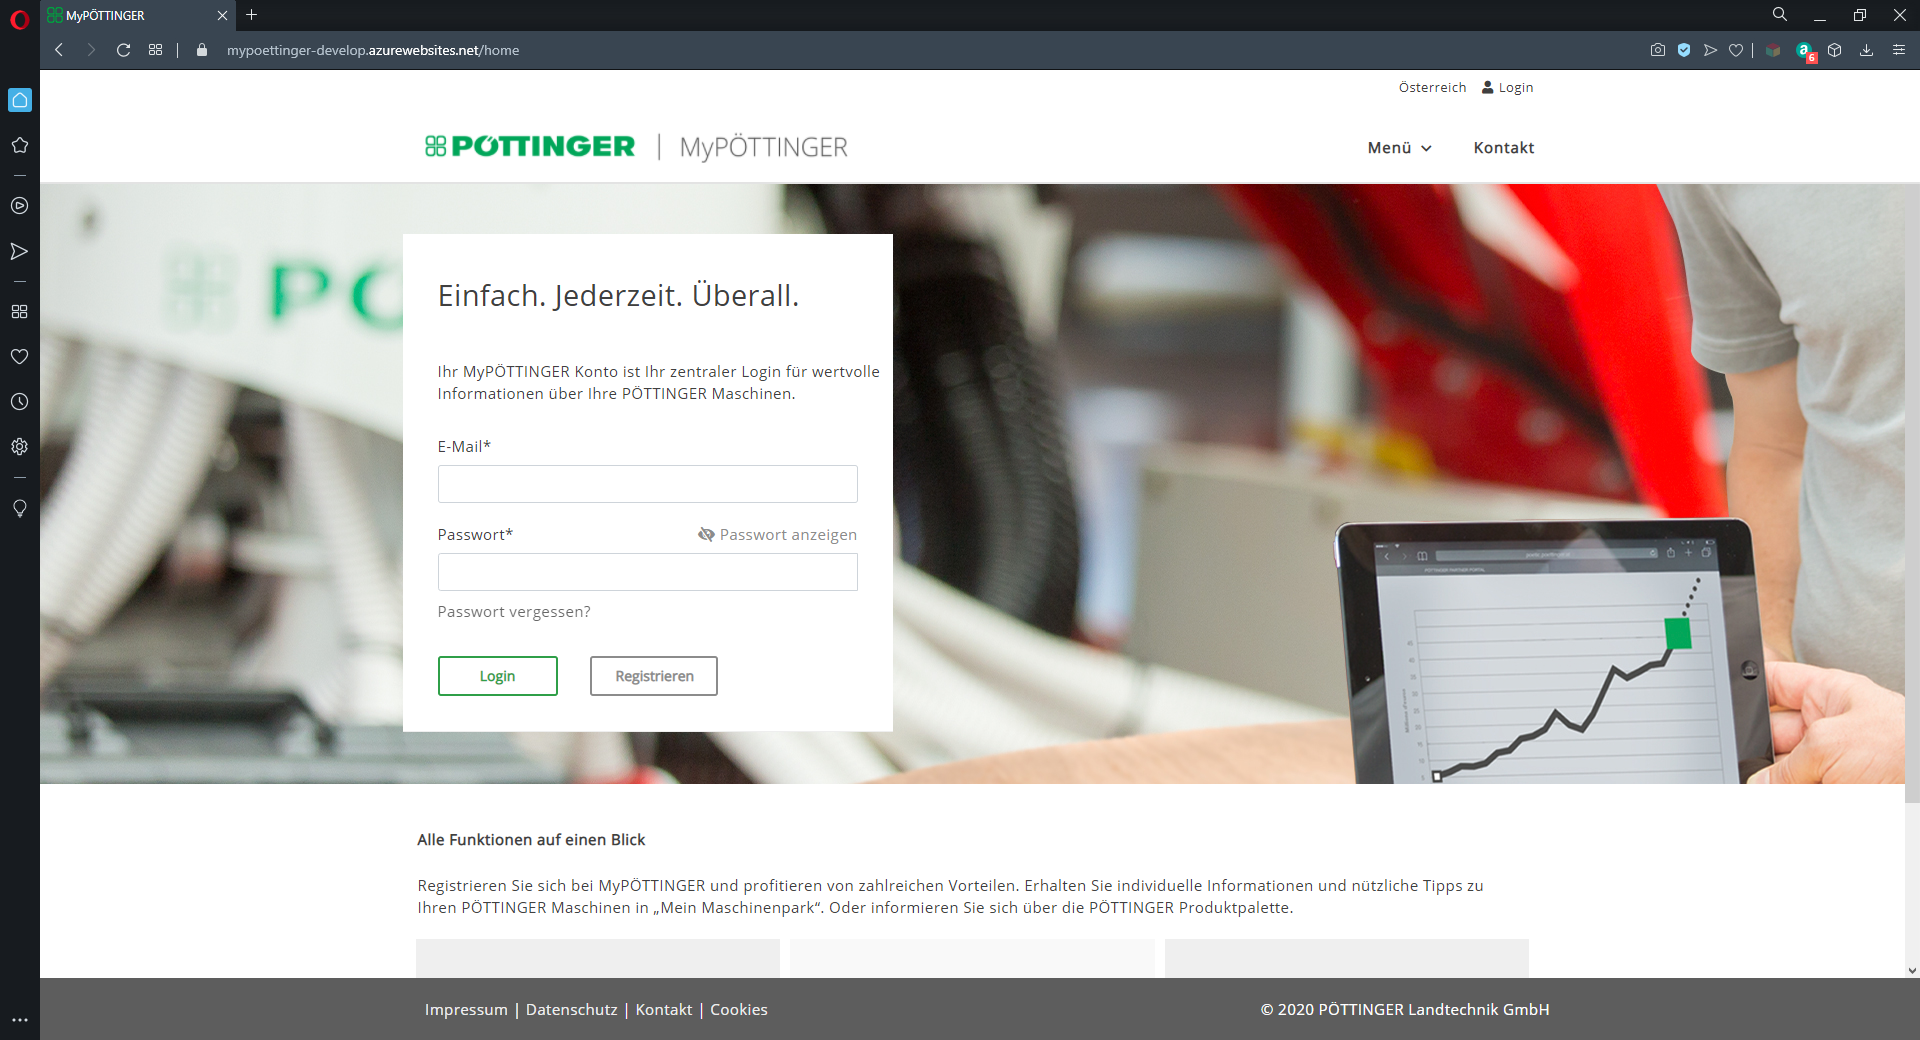
\includegraphics[width=0.8\textwidth]{./grafiken/erm_home_not_logged_in.png}
	}
	\vskip0pt
	\caption{Screenshot von der Startseite nicht eingeloggt} \label{fig:homeNotLoggedIn}
\end{figure}
\begin{figure}[H]
	\centerline{
		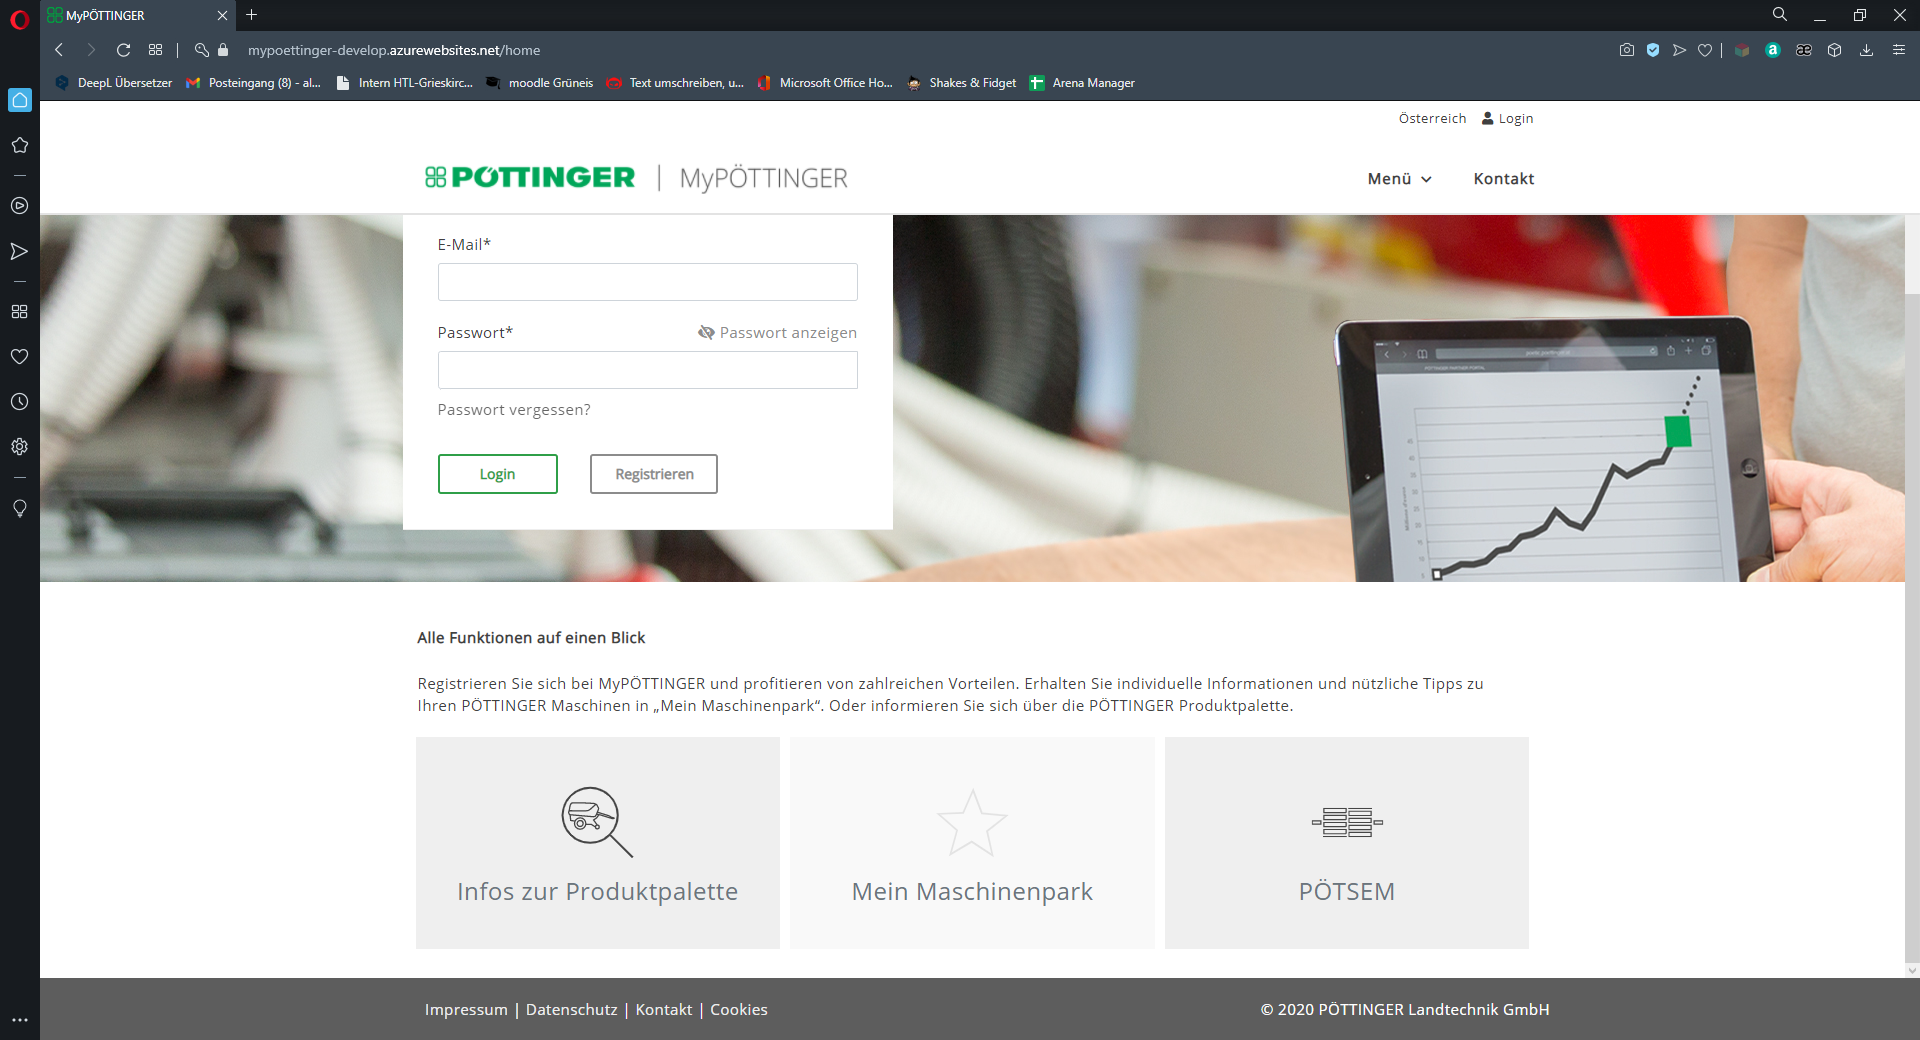
\includegraphics[width=0.8\textwidth]{./grafiken/erm_home_not_logged_in_2.png}
	}
	\vskip0pt
	\caption{Zweiter Screenshot von der Startseite nicht eingeloggt} \label{fig:homeNotLoggedIn2}
\end{figure}
Nach der Länderwahl gelangt man zu der Startseite. Anfangs ist man noch nicht eingeloggt, daher ist ein Login-Feld in der Mitte. Am zweiten Screenshot sieht man, dass das Feld "Mein Maschinenpark" etwas heller ist als die anderen Felder, da man den Maschinenpark nur als eingeloggter Benutzer nutzen kann. Die zwei anderen Felder sind auch ohne Registrierung nutzbar.
 
\subsection{Startseite nach dem Login}
\begin{figure}[H]
	\centerline{
		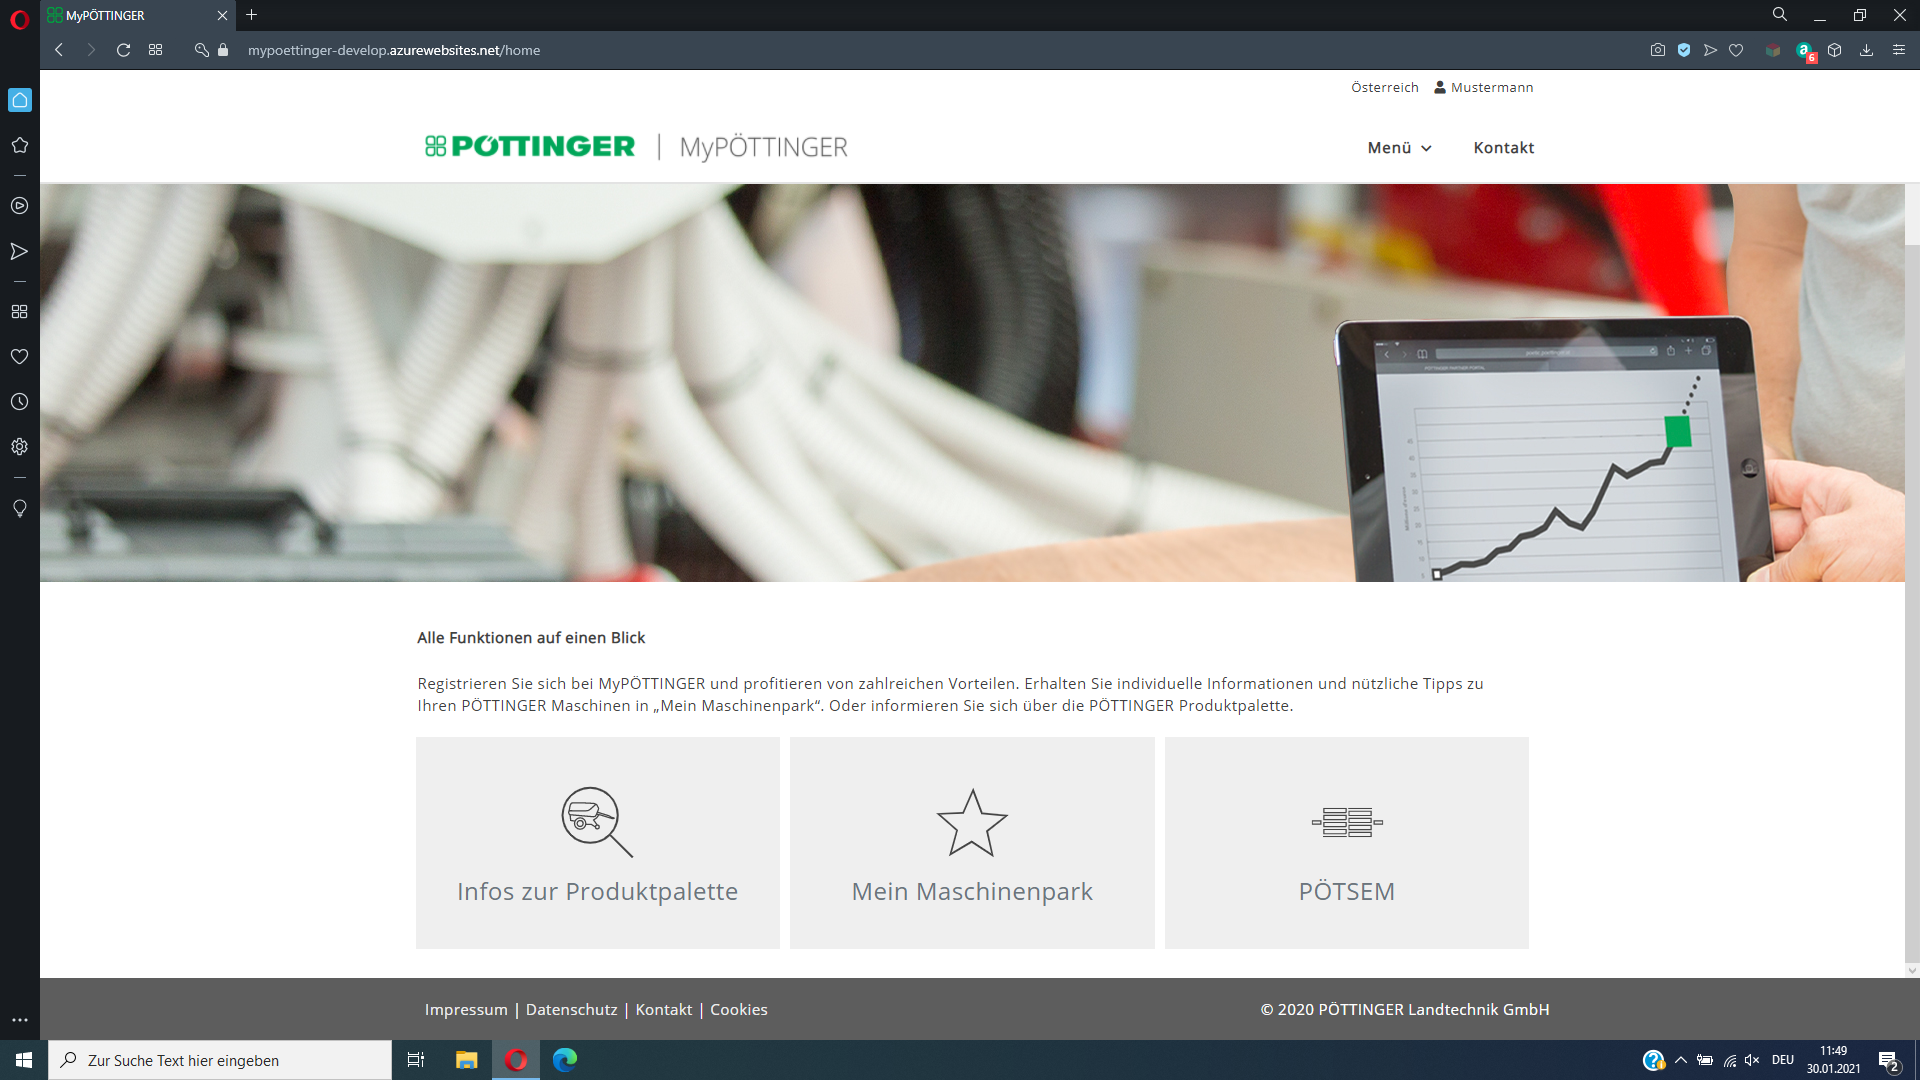
\includegraphics[width=0.8\textwidth]{./grafiken/erm_home_logged_in.png}
	}
	\vskip0pt
	\caption{Screenshot von der Startseite eingeloggt} \label{fig:homeLoggedIn}
\end{figure}
Nach dem Login ist das Feld "Mein Maschinenpark" aktiv. Als eingeloggter Benutzer hat man Zugriff auf den Maschinenpark. 
\section{Registrierungsseite}
Falls man noch nicht registriert ist und man auf der Startseite auf "Registrieren" drückt, wird man zur Registrierungsseite weitergeleitet.
\subsection{Registrierung}
\begin{figure}[H]
	\centerline{
		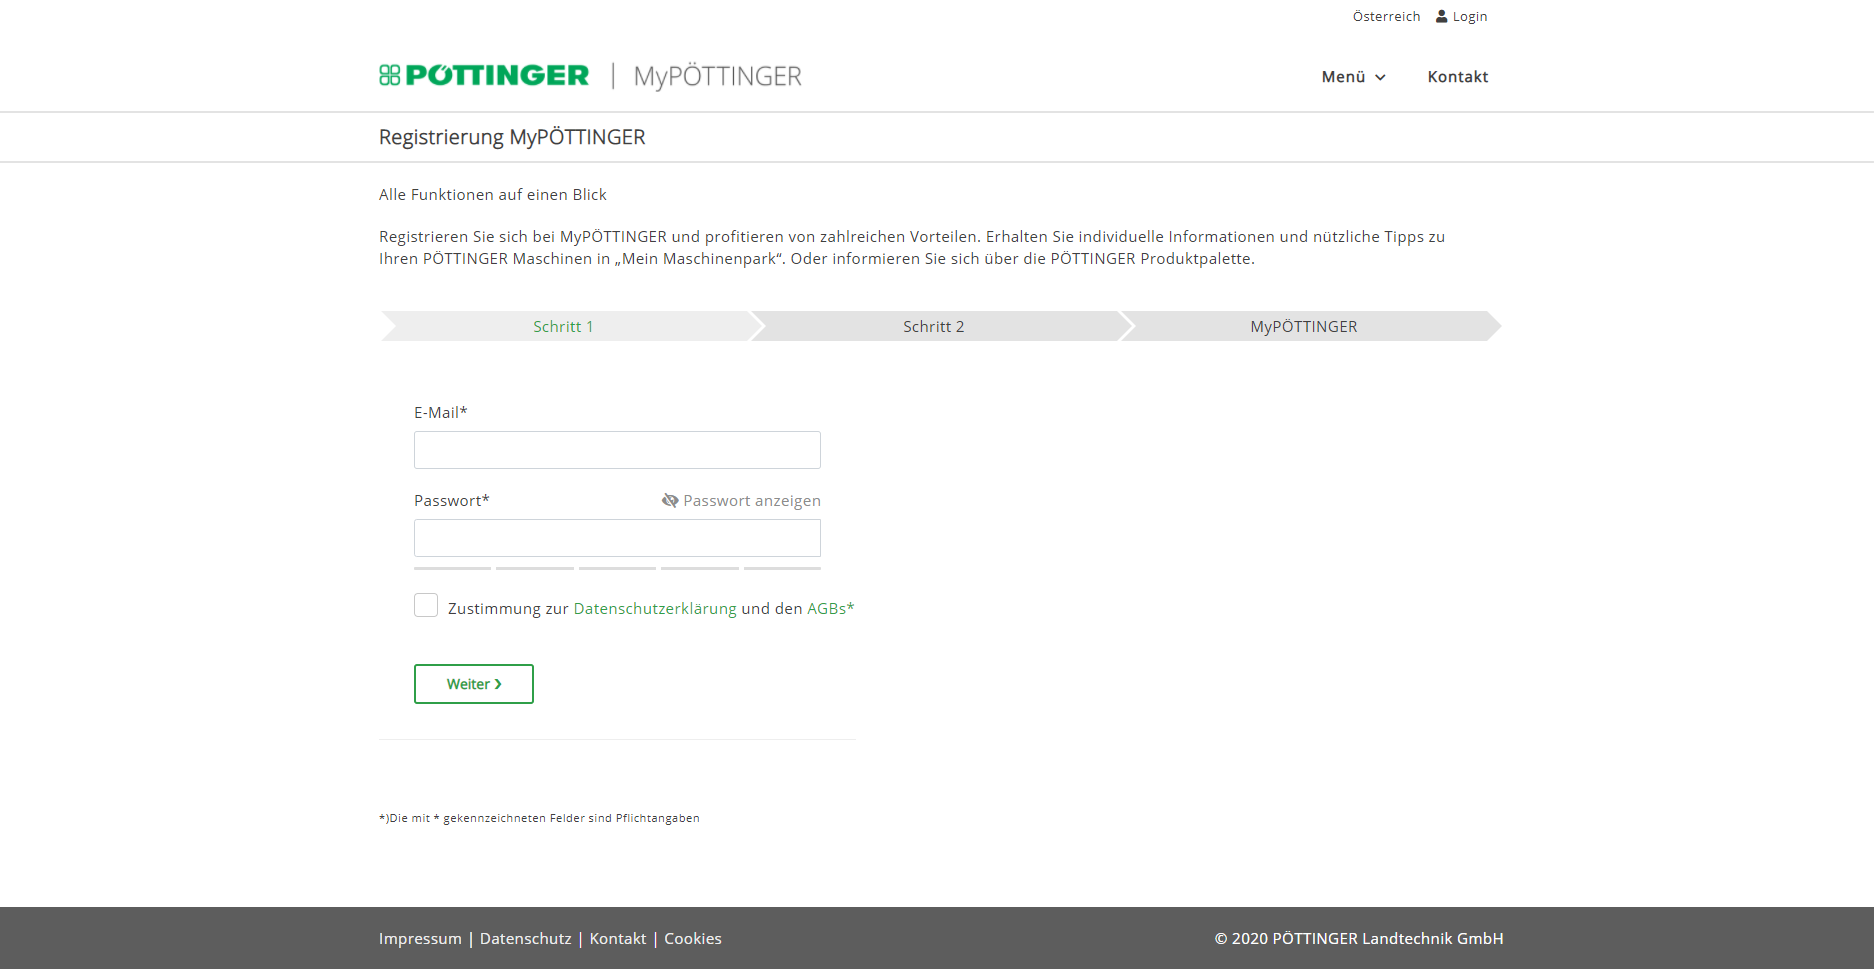
\includegraphics[width=0.8\textwidth]{./grafiken/erm_register.png}
	}
	\vskip0pt
	\caption{Screenshot von der Registrierungsseite} \label{fig:register}
\end{figure}
Während der Passworteingabe bekommt man Feedback, wie sicher das ausgewählte Passwort ist und was noch fehlt, um den Passwortanforderungen zu entsprechen. Die Passwortanforderungen entsprechen den Voraussetzungen von Auth0, da die Registrierung über Auth0 läuft. Der Balken unter dem Passwortfeld gibt die Sicherheit des Passwortes an. Das Passwort wird mit gängigen Namen und Nachnamen aus Amerika, beliebte englische Wörter und Muster wie Datumsangaben, Wiederholungen und Tastaturmuster verglichen um die Stärke angeben zu können.
\begin{figure}[H]
	\centerline{
		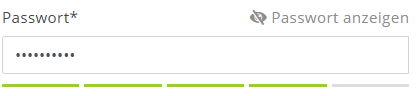
\includegraphics[width=0.8\textwidth]{./grafiken/passwordSecurity.PNG}
	}
	\vskip0pt
	\centerline{
		
\includegraphics[width=0.8\textwidth]{./grafiken/passwordHints.PNG}
	}
	\caption{Screenshot von der Passworteingabe} \label{fig:pw}
\end{figure}
\subsection{Weitere Daten für die Registrierung}
In diesem Schritt der Registrierung füllt man persönliche Daten aus. Das Land und die Sprache werden von der am Beginn ausgewählten Locale übernommen. Diese kann man aber auch hier ändern. Wenn das Land oder die Sprache geändert wird, wird dieses Formular neu generiert und die Felder werden nach dem Standard des Landes erzeugt. Das bedeutet, dass die Reihenfolge der angezeigten Felder von dem ausgewählten Land abhängt, da in gewissen Ländern der Nachname vor dem Vornamen in einem Formular steht. Die Feldbeschreibung wird auch nach der ausgewählten Sprache geändert. Weiters wird auch die Validierung der Felder geändert, denn die Postleitzahl in den verschiedenen Länder variiert. (4-stellig in Österreich, 5-stellig in Deutschland)\\

Für die Adresseingabe hat der Benutzer 3 Möglichkeiten:
Es besteht die Möglichkeit, jedes Adressfeld selber auszufüllen. Somit sind die Felder Straße und Hausnummer, Ort, Postleitzahl und bei gewissen Ländern die Provinzen oder Staaten auszufüllen.\\

Eine etwas schnellere Variante ist die Verwendung von dem integrierten Typeaheads. Bei der Eingabe des Feldes Straße und Hausnummer erscheinen Adresseingabevorschläge darunter. Wenn man auf die gewünschte Adresse klickt, werden die Felder Ort, Postleitzahl und falls vorhanden die Provinz oder der Staat automatisch ausgefüllt.\\

Die schnellste Variante ist die Verwendung von der integrierten Standorterkennung. Dafür drückt man den "Use my location" über dem Adressfeld. Dadurch wird der Standort bestmöglich erkannt und alle vorhandenen Adressfelder werden automatisch ausgefüllt. Falls der Standort nicht ganz richtig erkannt wurde, kann man es danach noch bearbeiten. Die Standorterkennung ändert auch das ausgewählte Land, falls diese nicht übereinstimmen.
\begin{figure}[H]
	\centerline{
		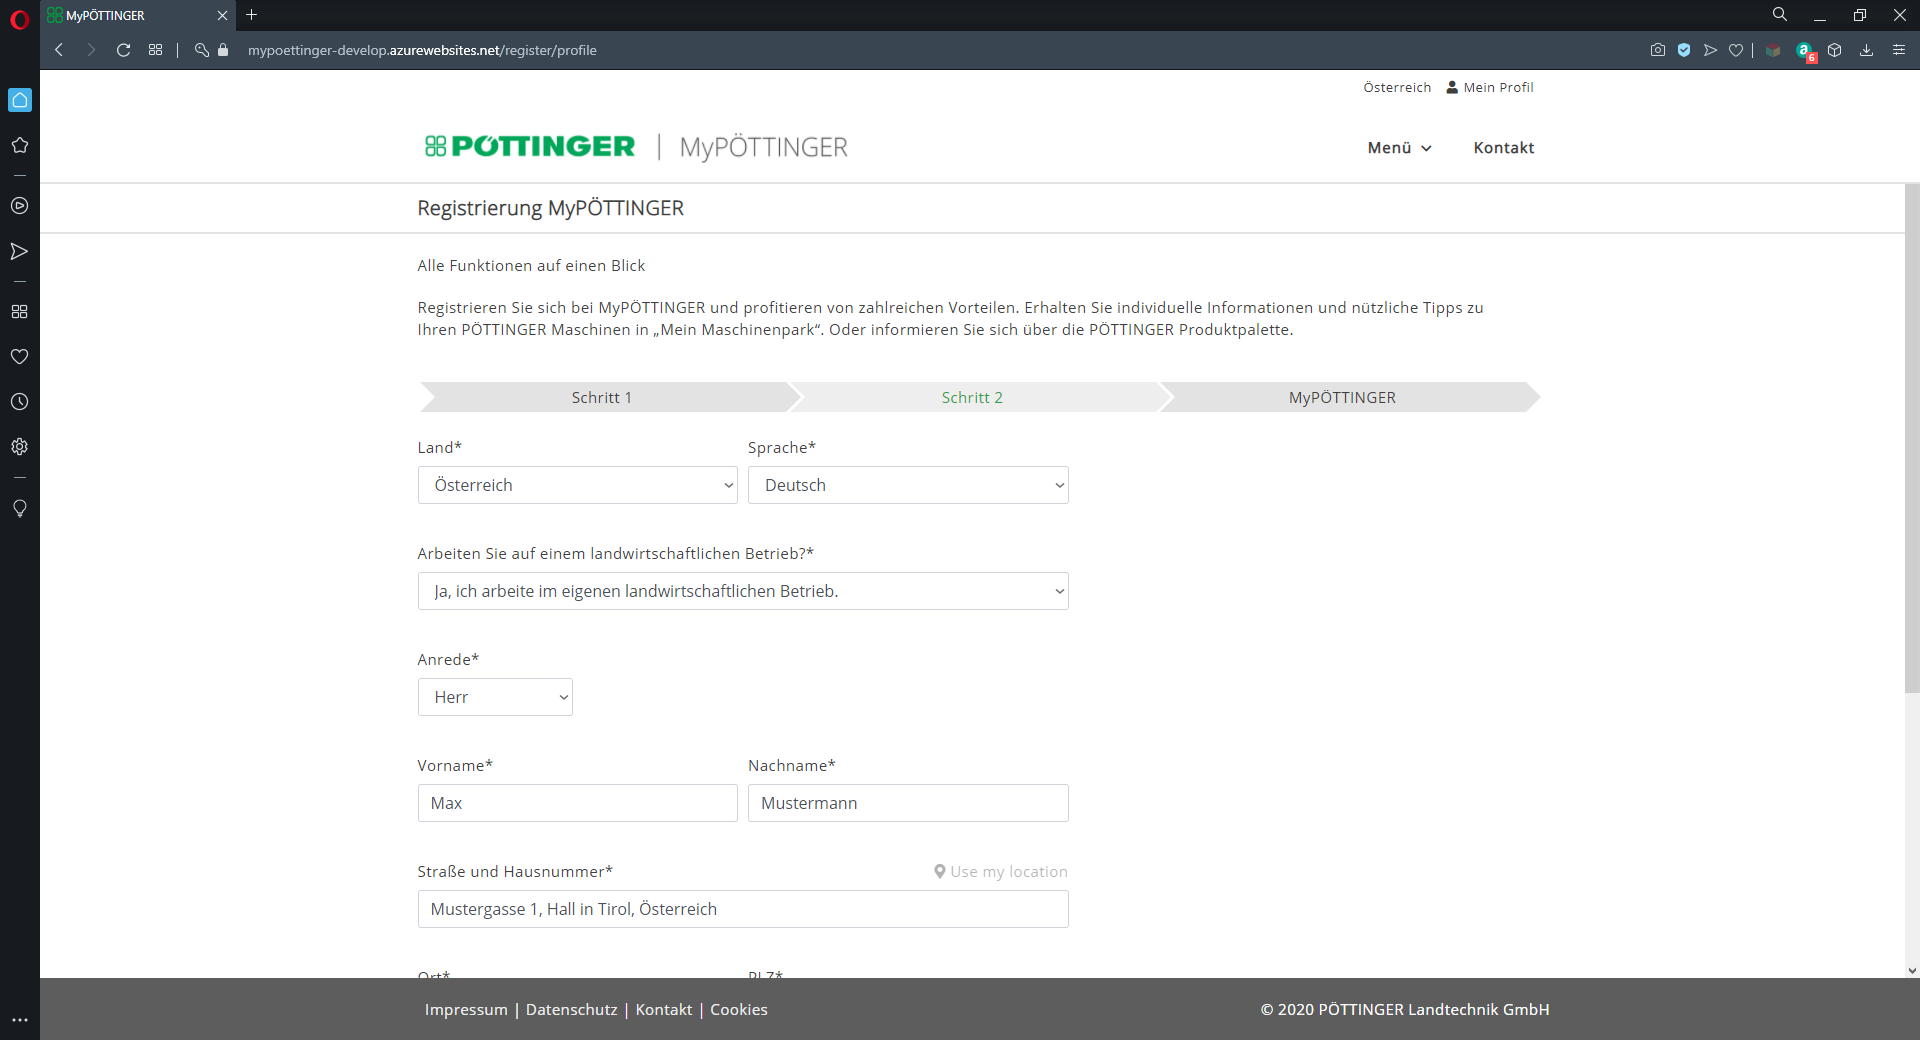
\includegraphics[width=0.8\textwidth]{./grafiken/erm_register_2.png}
	}
	\vskip0pt
	\caption{Screenshot von der Dateneingabe der Registrierung} \label{fig:register2}
\end{figure}
\begin{figure}[H]
	\centerline{
		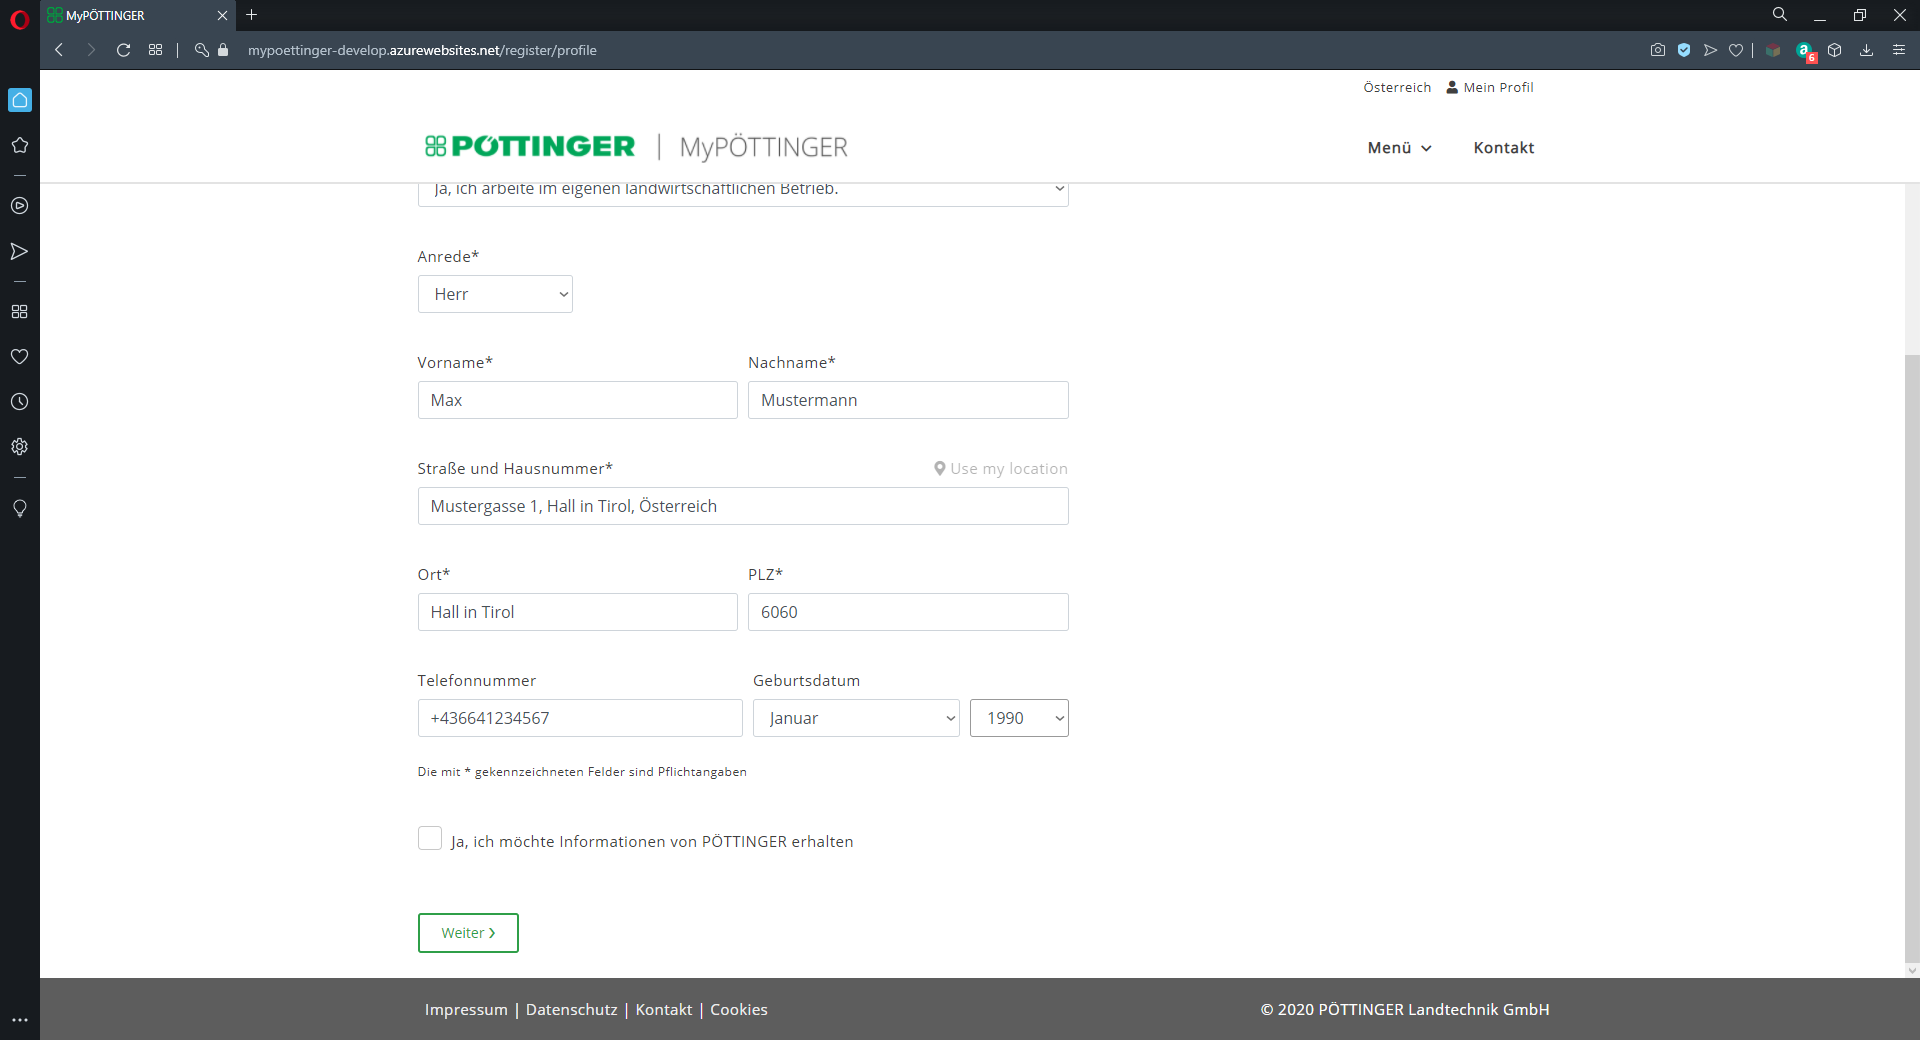
\includegraphics[width=0.8\textwidth]{./grafiken/erm_register_3.png}
	}
	\vskip0pt
	\caption{Zweiter Screenshot von der Dateneingabe der Registrierung} \label{fig:register3}
\end{figure}

Der Benutzer muss angeben, ob er auf dem eigenen landwirtschaftlichen Betrieb arbeitet, auf einem anderen landwirtschaftlichen Betrieb angestellt ist oder dass er auf keinen Betrieb arbeitet. Falls der Benutzer auswählt, dass er auf einen anderen Betrieb angestellt ist, erscheint zusätzlich das Feld für den Namen des Unternehmens.\\

Jedes Eingabefeld wird sofort nach Abgabe des Cursorfokus validiert. Falls ein Fehler auftritt wird das Feld rot umrandet und unter dem Feld erscheint eine Fehlermeldung, was falsch ist. Die Eingaben werden im Frontend und im Backend validiert. Im folgenden Screenshot sieht man die Felder mit einigen möglichen Fehlermeldungen.
\begin{figure}[H]
	\centerline{
		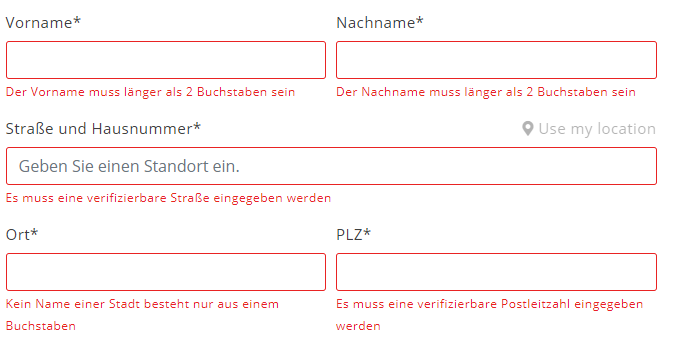
\includegraphics[width=0.8\textwidth]{./grafiken/dateneingabe_Errors.PNG}
	}
	\vskip0pt
	\caption{Screenshot von den Fehlermeldungen der Eingaben} \label{fig:eingabeError}
\end{figure}

\subsection{Letzter Schritt der Registrierung}
Um die Registrierung erfolgreich abzuschließen, bekommt man eine Bestätigung per E-Mail zugesendet. Darin befindet sich ein Aktivierungslink. Diese Seite sieht wie folgt aus:
\begin{figure}[H]
	\centerline{
		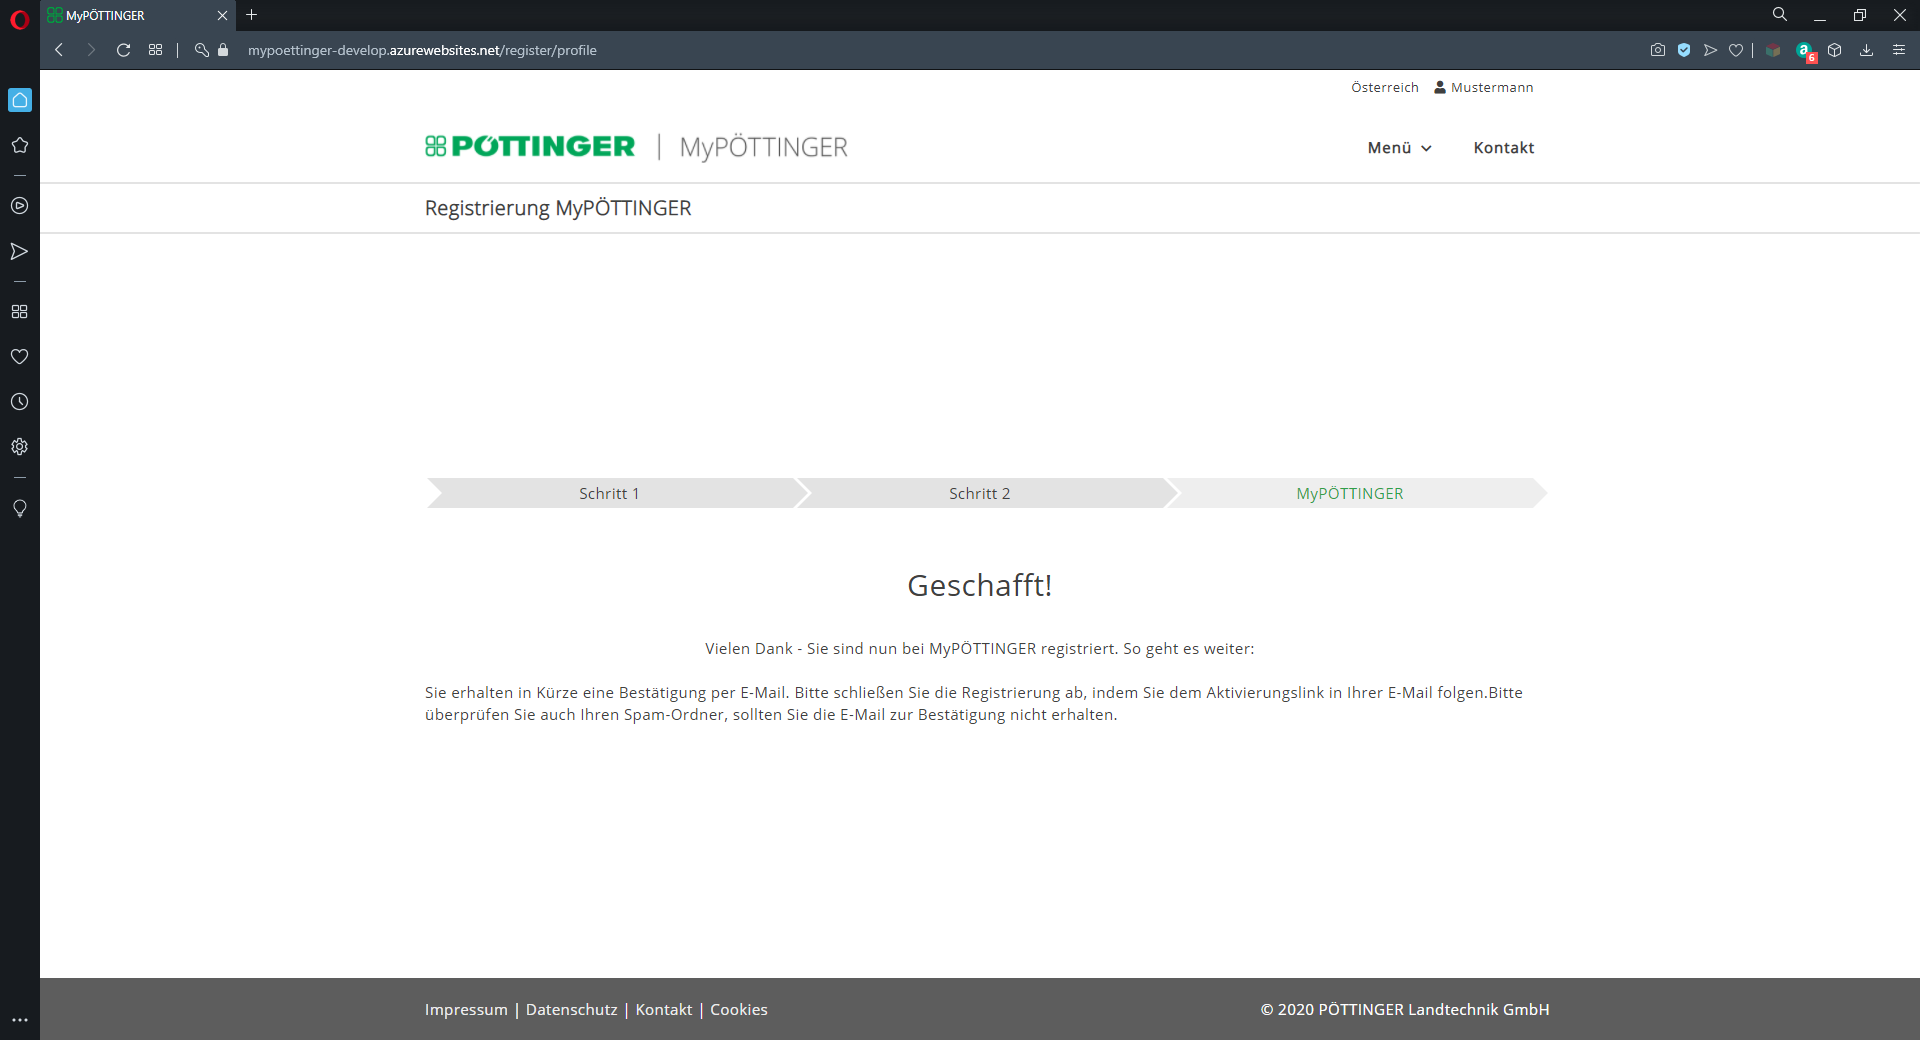
\includegraphics[width=0.8\textwidth]{./grafiken/erm_register_4.png}
	}
	\vskip0pt
	\caption{Screenshot von dem letzten Schritt der Registrierung} \label{fig:step3register}
\end{figure}

Nach der Bestätigung in der E-Mail kommt man wieder zurück auf die Startseite und es erscheint ein Pop-Up.
\begin{figure}[H]
	\centerline{
		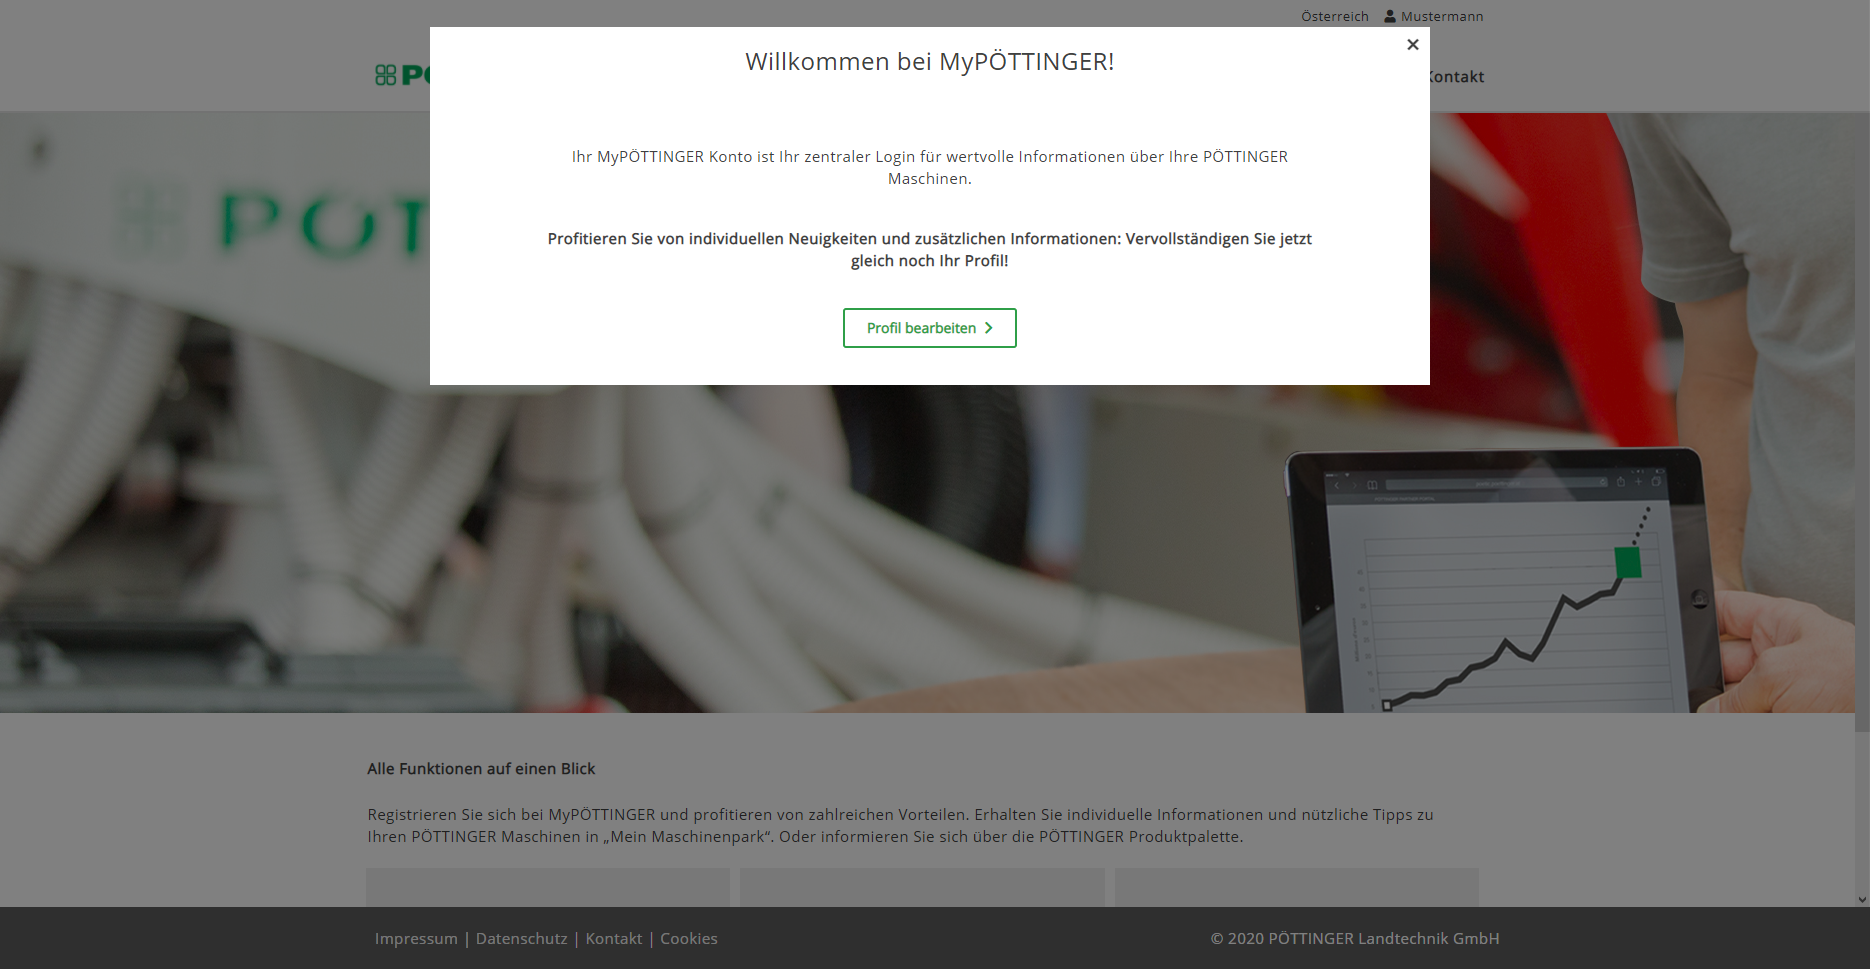
\includegraphics[width=0.8\textwidth]{./grafiken/erm_home_after_email.png}
	}
	\vskip0pt
	\caption{Screenshot von dem Bestätigungs-Pop-Up} \label{fig:popup}
\end{figure}

\section{Profilübersicht}
Auf die Profilübersicht gelangt man, wenn man in dem Bestätigungs-Pop-Up auf "Profil bearbeiten" klickt oder man klickt auf den eigenen Namen rechts oben und danach auf "Mein Profil". Die Profilübersicht sieht folgendermaßen aus:
\begin{figure}[H]
	\centerline{
		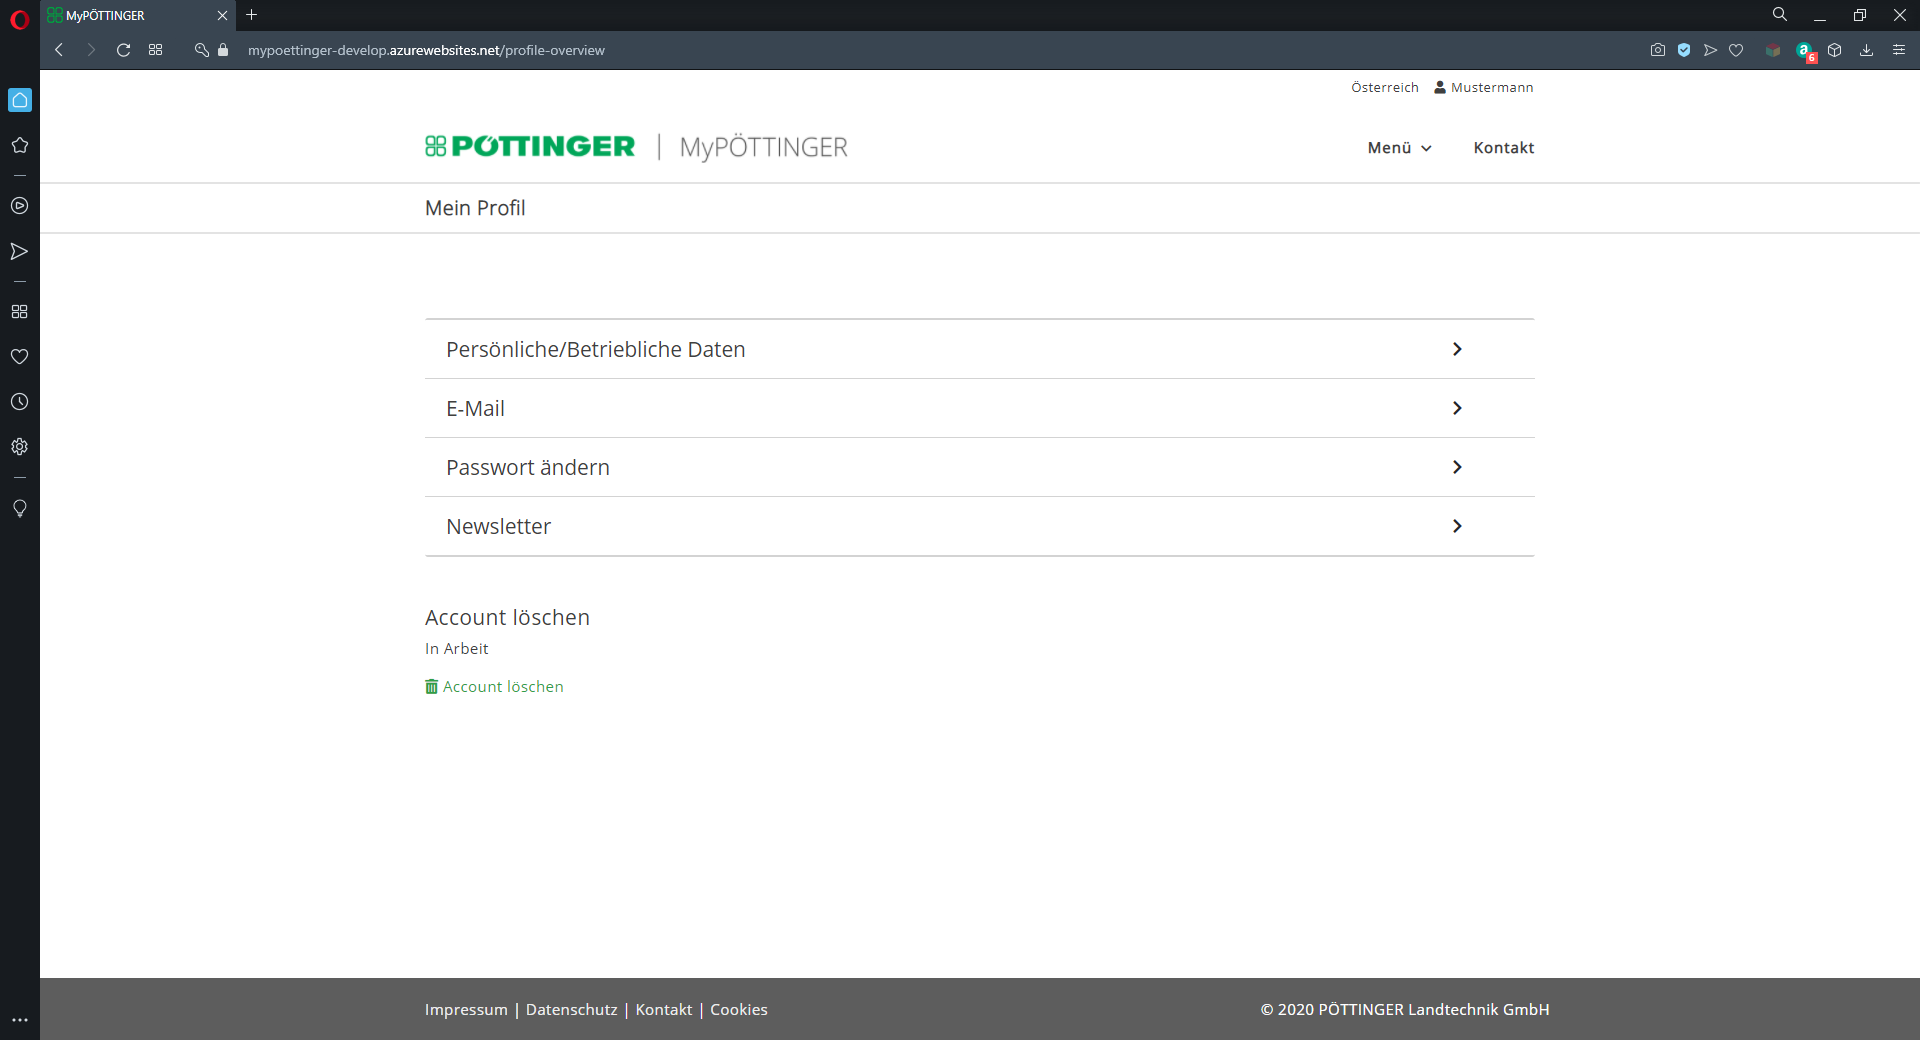
\includegraphics[width=0.8\textwidth]{./grafiken/erm_profil.png}
	}
	\vskip0pt
	\caption{Screenshot von der Profilübersicht} \label{fig:profil}
\end{figure}
In der Profilübersicht kann man all seine persönlichen Daten einsehen und diese auch bearbeiten.

\subsection{Persönliche/Betriebliche Daten}
Nach der Registrierung ist es möglich, hier noch weiter persönliche und betriebliche Daten einzutragen. Falls der Benutzer ausgewählt hat, dass er auf dem eigenen oder einem anderen landwirtschaftlichen Betrieb arbeitet, erweitern sich die Daten um einige Felder für den Betrieb. Bei einem Klick auf "Persönliche/Betriebliche Daten" klappt sich ein Datenformular auf, dass wie folgt aussieht:
\begin{figure}[H]
	\centerline{
		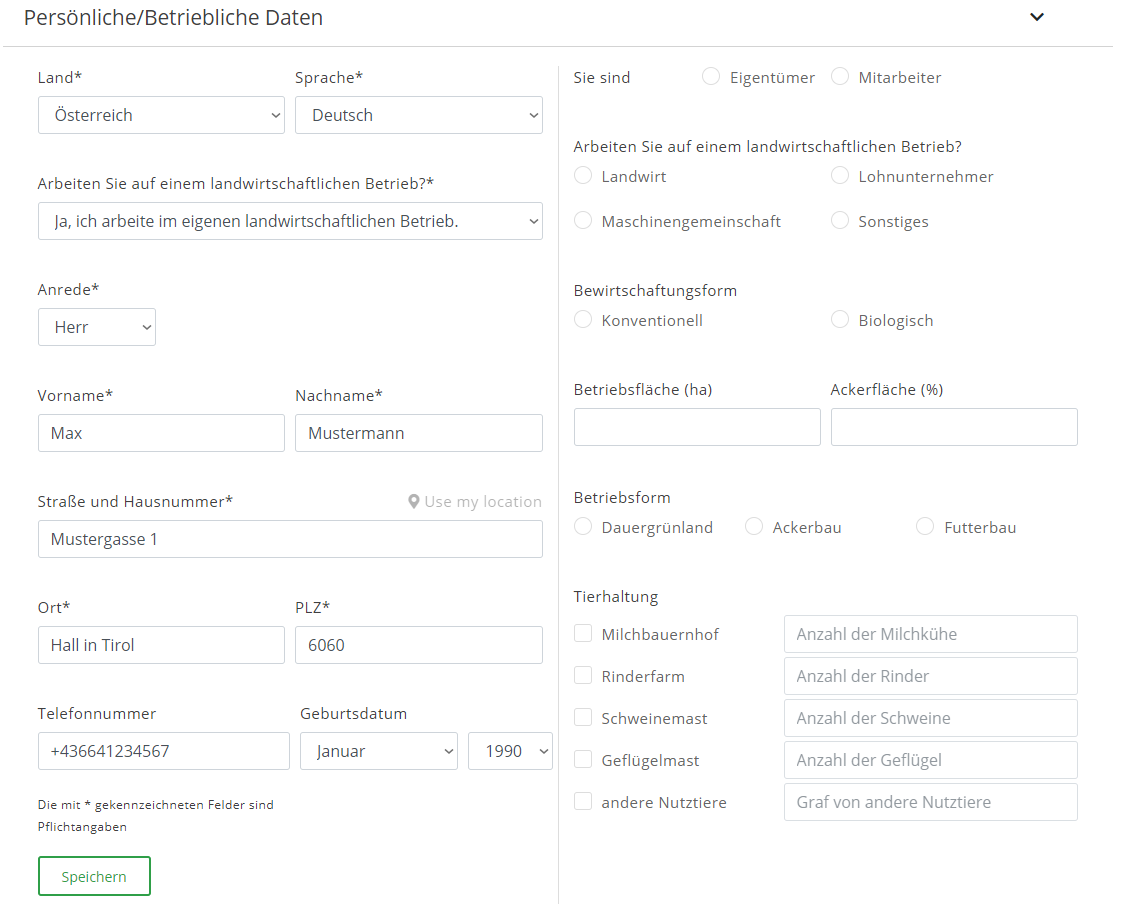
\includegraphics[width=\textwidth]{./grafiken/erm_profil_daten.png}
	}
	\vskip0pt
	\caption{Persönliche/Betriebliche Daten} \label{fig:profilData}
\end{figure}



